% ============================================================
%  第一章 周期性结构（§1–§5 + 章末参考文献）
%  底本：高等教育出版社《固体理论》（第二版）印刷页 1–17（PDF p021–p037）
%  OCR 输入：MinerU/full_merged.md 行 433–1141
%  公式编号自检：§1 (1.1.1)–(1.1.8)；§1 脚注① (1.1.9)–(1.1.10)；
%    §2 (1.2.1)–(1.2.3)；§3 (1.3.1)–(1.3.23)；§4 (1.4.1)–(1.4.16)；
%    §5 (1.5.1)–(1.5.22)。全部自动编号，逐一对上。
%  已修正的 OCR/原书错误：
%  1. L445 句子截断："…作为基矢 a_i(i)=1 图…/2,3)，如图1.1中…"，
%     按原书 p021 复原为"…作为基矢 a_i(i=1,2,3)，如图1.1中左下角的取法…"
%  2. (1.1.4) 被拆成相邻两个 $$ 块（b1,b2 无号 + b3 带号），按原书 p022
%     合并为一个编号公式
%  3. (1.1.3) OCR 作 a_i·b_i=2π\hatδ_ij，原书为 a_i·b_j=2πδ_ij（cases 形式），
%     右端"(i,j=1,2,3)"照录；\hat{δ}→δ
%  4. (1.1.5) 末尾 OCR 乱码"(n_i=def def=∅)"，原书为"(n_i=整数)"；
%     (1.1.8) 乱码"(m=整数)"同此复原
%  5. §1 脚注①（含编号公式 (1.1.9)、(1.1.10)）整段被 OCR 漏失，
%     按原书 p023 页脚补录，公式仍用自动编号得 (1.1.9)/(1.1.10)
%  6. "即平等算符之间可对易"：原书 p024 排印错误，"平等"→"平移"
%  7. (1.3.3) OCR tag 残缺为 \tag{.3}、公式内容乱码，原书 p025 有此式
%     （三行，ψ(r) 基函数），非原书跳号；已按原书补排，编号自动复原
%  8. §3 中 φ(r)/ψ(r) 混排处按原书统一为 ψ(r)（含 (1.3.3)–(1.3.6)、
%     (1.3.9a)、(1.4.9) 等）
%  9. (1.3.9a) 为原书自带的二级编号，自动编号无法产生，唯一例外采用
%     equation* + \tag{1.3.9a} 照录，不计入自动编号序列
% 10. (1.3.14) χ^{(⋆)}/D^{(⋆)} 原书为 χ^{(k)}/D^{(k)}
% 11. "每一许可k值所占据的体系为"：OCR 键错，原书 p027 为"体积"
% 12. "但必未就是点阵"→"但未必就是点阵"（原书 p030 为"未必"，OCR 键错）
% 13. "群元{β|τ_β}这时"→按原书补逗号"群元{β|τ_β}，这时"
% 14. "布洛赫定理式(1.3.9)]"→"[式(1.3.9)]"（补左方括号）
% 15. ψ_{n⋆}(k,r)→ψ_{n↑}(k,r)；r→r、k→(−k)、ŝ→(−ŝ) 箭头按原书复原
% 16. 时间反演段"E_{n↑}(k)=E_{n↑}(−k)、E_{n↓}(k)=E_{n↓}(−k)"OCR 乱码，
%     按原书 p034 复原（顿号相连）
% 17. (1.5.6) OCR 残缺"f_K=Ω^{-1/2}|_Ω f…"，按原书 p035 复原
% 18. (1.5.7) 末行乱码"(当 k=K 倒格矢时)/(当 k≠K 时)"按原书复原
% 19. (1.5.3) 原书 δ_{k,o} 下标排印为字母 o，按物理更正为 δ_{k,0}
% 20. "可称为周期函数的格林定 Ω 理"→"格林定理"（OCR 串入 Ω）
% 21. 文献[3] "New York; John Wiley"→"New York: John Wiley"（按原书 p037）
% 22. 其余：全角句点"．"→"."；删除 OCR 间隔符"~"；\mathrm{d} 收紧；
%     {E|α}-1 型花括号残缺按原书补全；群论正交关系中 δ_{γσ̂}→δ_{γδ}、
%     \widetildeΘ/\widehatΩ→δ、Σk∈nZ→Σk∈BZ 等公式噪声修正
%  遗留问题：图 1.1–1.8 均为占位图（fig1-N.pdf），宽度按原书目测配置
% ============================================================
\chapter{周期性结构}

\section{正格矢与倒格矢}

晶体的第一重要特征是原子（离子或分子）排列的周期性.几何上可用点阵表现晶体结构的周期性，点阵中任一格点的位置由正格矢决定：
\begin{equation}
  \boldsymbol{R}_l=l_1\boldsymbol{a}_1+l_2\boldsymbol{a}_2+l_3\boldsymbol{a}_3
  =\sum_{i=1}^{3}l_i\boldsymbol{a}_i
\end{equation}
其中 $l_1$、$l_2$、$l_3$ 取所有整数.$\boldsymbol{a}_1$、$\boldsymbol{a}_2$、$\boldsymbol{a}_3$ 为点阵的基矢（或称初基平移），它们构成的平行六面体叫元胞（或初基元胞），元胞是点阵的最小重复单元，每个元胞中平均只包含一个格点.显然，元胞和基矢的选择并非唯一.以二维点阵作例，图1.1中的4种取法都能保证经基矢的整数平移到达任一格点，这4种元胞也都只含一个格点.为了简单起见，常取尽可能短的矢量作为基矢 $\boldsymbol{a}_i\,(i=1,2,3)$，如图1.1中左下角的取法，于是也相应地确定了元胞（图中斜线区）.

\begin{center}
\begin{minipage}{6.5cm}
\centering
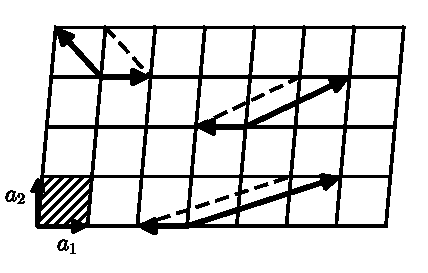
\includegraphics[width=6.5cm]{fig1-1.pdf}\\{\small 图 1.1\quad 二维点阵的元胞和基矢}
\end{minipage}
\end{center}

在三维情况下，元胞的体积为
\begin{equation}
  \Omega=\boldsymbol{a}_1\cdot(\boldsymbol{a}_2\times\boldsymbol{a}_3)
\end{equation}
应当指出，在固体物理学中还采用另一种外形较复杂的元胞.它是由一个格点与最近邻格点（有时也包括次近邻）的连线中垂面所围成的多面体，其中只包含一个结点，称为维格纳—赛茨元胞（简称W-S元胞），如图1.2所示.二维六角点阵的W-S元胞为正六边形，它比 $\boldsymbol{a}_1$、$\boldsymbol{a}_2$ 所组成的初基元胞更明显地反映出点阵的对称性.在三维情况下，简立方（sc）点阵的W-S元胞仍为立方体，体心立方（bcc）点阵的W-S元胞为截角八面体，面心立方点阵（fcc）则为菱十二面体，如图1.3所示.显然，W-S元胞是对称性元胞，它具有所属点阵点群的全部对称性.一切保持点阵不变的旋转、反射和反演操作都将同时保持W-S元胞不变，这为理论计算将带来方便.

\begin{center}
\begin{minipage}{5.5cm}
\centering
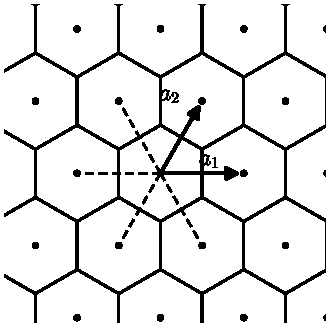
\includegraphics[width=5.5cm]{fig1-2.pdf}\\{\small 图 1.2\quad 二维六角点阵的W-S元胞}
\end{minipage}
\end{center}

由于晶体中的电子、声子、自旋波量子等元激发的状态都是用波矢量描述的，为便于讨论问题，又在波矢量空间人为地引入另一套点阵，称为倒点阵，它的长度量纲是坐标空间中长度量纲的倒数.倒点阵的基矢 $\boldsymbol{b}_i\,(i=1,2,3)$ 是由晶体点阵的基矢 $\boldsymbol{a}_i$ 按下列关系式定义的：
\begin{equation}
  \boldsymbol{a}_i\cdot\boldsymbol{b}_j=2\pi\delta_{ij}
  =\begin{cases}2\pi&(i=j)\\0&(i\neq j)\end{cases}
  \qquad(i,j=1,2,3)
\end{equation}

\begin{center}
\begin{minipage}{10.5cm}
\centering
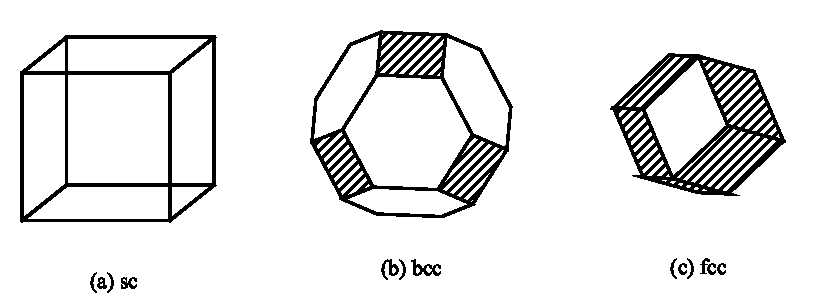
\includegraphics[width=10.5cm]{fig1-3.pdf}\\{\small 图 1.3\quad sc、bcc、fcc 点阵的W-S元胞}
\end{minipage}
\end{center}

容易求出 $\boldsymbol{b}_i$ 为
\begin{equation}
  \boldsymbol{b}_1=\frac{2\pi}{\Omega}(\boldsymbol{a}_2\times\boldsymbol{a}_3)\text{，}\quad
  \boldsymbol{b}_2=\frac{2\pi}{\Omega}(\boldsymbol{a}_3\times\boldsymbol{a}_1)\text{，}\quad
  \boldsymbol{b}_3=\frac{2\pi}{\Omega}(\boldsymbol{a}_1\times\boldsymbol{a}_2)
\end{equation}
在倒点阵中任一格点的位置矢
\begin{equation}
  \boldsymbol{K}_n=n_1\boldsymbol{b}_1+n_2\boldsymbol{b}_2+n_3\boldsymbol{b}_3
  =\sum_{i=1}^{3}n_i\boldsymbol{b}_i\qquad(n_i=\text{整数})
\end{equation}
称为倒格矢.与正点阵相似，倒点阵基矢 $\boldsymbol{b}_1$、$\boldsymbol{b}_2$、$\boldsymbol{b}_3$ 组成的平行六面体是倒点阵的元胞，它等于
\begin{equation}
  \Omega^{*}=\boldsymbol{b}_1\cdot(\boldsymbol{b}_2\times\boldsymbol{b}_3)
\end{equation}
为了便于讨论晶体对称性对电子、声子等能谱结构的影响，通常取倒点阵中相应的W-S元胞作为倒点阵的元胞.它是相对倒格点对称配置的多面体，在此多面体边界面上的任一点可由边界面上另一点加上一个倒格矢 $\boldsymbol{K}_n$ 的平移达到.当这个多面体的中心定为倒易空间的原点时，它所包含的区域称为第一布里渊区，用BZ表示，又称简约区.

倒点阵是根据正点阵作出的，它与正点阵有一一对应关系，其中正、倒点阵的元胞体积关系
\begin{equation}
  \Omega\Omega^{*}=(2\pi)^3
\end{equation}
和正、倒格矢之间的
\begin{equation}
  \boldsymbol{K}_n\cdot\boldsymbol{R}_l=2\pi\sum_{i=1}^{3}n_il_i=2\pi m
  \qquad(m=\text{整数})
\end{equation}
关系最为重要.

sc 正点阵的倒点阵仍为 sc，其 BZ 形状与图1.3(a)相同.fcc 正点阵的倒点阵为 bcc，其 BZ 形状如图1.3(b).bcc 正点阵的倒点阵为 fcc，其 BZ 形状与图1.3(c)同.

BZ是波矢量空间中的对称化元胞，它具有倒点阵点群的全部对称性，利用式(1.1.8)容易证明\footnote{其简单证明如下：设 $\alpha$ 为正点阵点群的对称操作，则 $\alpha\boldsymbol{R}_l$ 应为一个正格矢.由于群中有 $\alpha$ 必有逆操作 $\alpha^{-1}$，所以 $\alpha^{-1}\boldsymbol{R}_l$ 也应为一正格矢.根据式(1.1.8)应有
\begin{equation}
  \alpha^{-1}\boldsymbol{R}_l\cdot\boldsymbol{K}_n=2\pi m
\end{equation}
由于两矢量的点乘对于正交变换是不变的，上式可化为
\begin{equation}
  \boldsymbol{R}_l\cdot\alpha\boldsymbol{K}_n=2\pi m
\end{equation}
所以，对群中任意 $\alpha$ 而言，$\alpha\boldsymbol{K}_n$ 亦为一倒格矢，表明正、倒点阵具有相同点群对称性.}，同一晶体的正、倒点阵有相同的点群对称性，因此，可以简单地说，BZ具有晶体点阵点群的全部对称性.

\section{平移对称性}

点阵是格点在空间中的无限周期重复排列，点阵具有平移对称性，表现为将整体作任意正格矢的平移后，它将恢复原状；或者说，从空间任一点（并不一定是格点）出发，作任意正格矢的位移，必达到等效的点上.人们把晶体排列的周期性用抽象的几何点阵来表现，就是要赋予晶体平移不变的特征，使得含有大数粒子的完整晶体问题容易处理.平移对称性在固体物理学中占有十分重要的地位.

严格讲，只有无限理想晶体才具有平移对称性，实际晶体的尺寸都是有限的，边界面的存在必然会破坏平移对称性.但是，考虑到大块晶体的尺寸（如 $1\,\mathrm{cm}=10^{7}\,\mathrm{nm}$）总是比元胞的边长（$0.1\sim1\,\mathrm{nm}$）大 $10^{7}\sim10^{8}$ 量级，晶体体内的总粒子数也相应地比表面上粒子数大相同的量级；因此，当研究大块晶体特性时，表面效应并不重要，大块晶体的属性近似与边界条件的选择无关，于是可以设计一种特殊的边界条件，使有限晶体也具有平移不变性，这就是玻恩—卡门边界条件提出的背景.他们把3边长为 $N_1\boldsymbol{a}_1$、$N_2\boldsymbol{a}_2$、$N_3\boldsymbol{a}_3$ 的有限晶体设想为沿 $\boldsymbol{a}_1$、$\boldsymbol{a}_2$、$\boldsymbol{a}_3$ 3个方向上首尾相衔接的“环”，这样的配置规定了从晶体内的任一点平移 $N_1\boldsymbol{a}_1$、$N_2\boldsymbol{a}_2$、$N_3\boldsymbol{a}_3$ 必将再返回原处.这是一个循环条件，它相当于把无限多个晶体“复本”毫无缝隙地拼合在一起，组成一个无限晶体，图1.4是其一维示意图，这样做就保证了有限晶体也具有平移对称性.玻恩—卡门循环边界条件在数学上归结为 $N_i\boldsymbol{a}_i\,(i=1,2,3)$ 的平移操作是恒等操作，
\begin{equation}
  \{E|N_i\boldsymbol{a}_i\}=\{E|N_i\boldsymbol{a}_i\}^{-1}=\{E|0\}
\end{equation}

\begin{center}
\begin{minipage}{5cm}
\centering
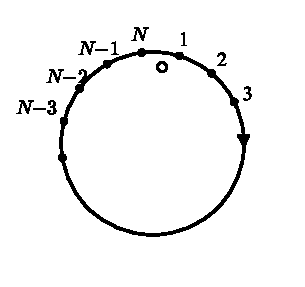
\includegraphics[width=5cm]{fig1-4.pdf}\\{\small 图 1.4\quad 波恩—卡门循环}
\end{minipage}
\end{center}

$\{E|\boldsymbol{R}_l\}$ 是平移算符，它对坐标的作用为
\begin{equation}
  \{E|\boldsymbol{R}_l\}\boldsymbol{r}=\boldsymbol{r}+\boldsymbol{R}_l\text{，}\quad
  \{E|\boldsymbol{R}_l\}^{-1}\boldsymbol{r}=\boldsymbol{r}-\boldsymbol{R}_l
\end{equation}
对函数的作用相应记为
\begin{equation}
\begin{aligned}
  \{E|\boldsymbol{R}_l\}f(\boldsymbol{r})
  &=f(\{E|\boldsymbol{R}_l\}^{-1}\boldsymbol{r})=f(\boldsymbol{r}-\boldsymbol{R}_l)\\
  \{E|\boldsymbol{R}_l\}^{-1}f(\boldsymbol{r})
  &=f(\{E|\boldsymbol{R}_l\}\boldsymbol{r})=f(\boldsymbol{r}+\boldsymbol{R}_l)
\end{aligned}
\end{equation}
对于元胞数为 $N=N_1N_2N_3$ 的晶体，共有 $N$ 个平移算符 $\{E|\boldsymbol{R}_l\}$，它们的集合满足群的组成条件：

(i) 任意两次相继的平移仍为一平移，即 $\{E|\boldsymbol{R}_1\}$ 乘 $\{E|\boldsymbol{R}_2\}$ 仍在 $\{E|\boldsymbol{R}_l\}$ 的集合之中.

(ii) 满足乘法的结合律.

(iii) 对每一个 $\{E|\boldsymbol{R}_l\}$，都存在 $\{E|\boldsymbol{R}_l\}^{-1}$，代表反方向的平移.$\{E|\boldsymbol{R}_l\}^{-1}$ 是 $\{E|\boldsymbol{R}_l\}$ 的逆元素.

(iv) 存在着恒等操作 $\{E|0\}$.

$\{E|\boldsymbol{R}_l\}$ 所组成的群叫平移群.平移群最重要的特征是相继两次平移的效果与它们作用的先后次序无关，即平移算符之间可对易，平移群是阿贝尔群.下面将讨论平移对称性对于晶体性能的影响.

\section{布洛赫定理}

当 $N\,(N=N_1N_2N_3)$ 个元胞的晶体满足玻恩—卡门条件时，具有平移对称性，其中正格矢 $\boldsymbol{R}_l=\sum_{i=1}^{3}l_i\boldsymbol{a}_i$ 可取 $N$ 个不同值，相应的有 $N$ 个平移算符 $\{E|\boldsymbol{R}_l\}$ 组成 $N$ 阶平移群.由于对所有的群元下列等式都成立，即
\begin{equation}
  \{E|\boldsymbol{R}_l\}^{-1}\{E|\boldsymbol{R}_m\}\{E|\boldsymbol{R}_l\}
  =\{E|\boldsymbol{R}_m\}
\end{equation}
故此 $N$ 阶群的每个元素本身自成一个共轭类.根据群论，群中共轭类数与不可约表示数相同.因此平移群有 $N$ 个不可约表示，不可约表示的维数 $n_\alpha$ 可由方程
\begin{equation}
  \sum_{\alpha=1}^{N}n_\alpha^2=N
\end{equation}
定出为 $n_\alpha\,(\alpha=1,2,\cdots,N)$，说明平移群的 $N$ 个不可约表示都是一维的.设 $\psi(\boldsymbol{r})$ 是此一维表示的基函数，则应有
\begin{equation}
\begin{aligned}
  &\{E|\boldsymbol{a}_j\}^{-1}\psi(\boldsymbol{r})
  =\psi(\{E|\boldsymbol{a}_j\}\boldsymbol{r})
  =\psi(\boldsymbol{r}+\boldsymbol{a}_j)
  =D(\{E|\boldsymbol{a}_j\})\psi(\boldsymbol{r})\\
  &\{E|\boldsymbol{a}_j\}^{-1}\{E|\boldsymbol{a}_j\}^{-1}\psi(\boldsymbol{r})
  =\{E|2\boldsymbol{a}_j\}^{-1}\psi(\boldsymbol{r})=D^2\psi(\boldsymbol{r})\\
  &\{E|N_j\boldsymbol{a}_j\}^{-1}\psi(\boldsymbol{r})
  =D^{N_j}\psi(\boldsymbol{r})\qquad(j=1,2,3)
\end{aligned}
\end{equation}
这里 $D$ 是表示的一维矩阵，实际上是一个数，利用循环边界条件式(1.2.1)得到
\begin{equation}
  D^{N_j}\psi(\boldsymbol{r})=\{E|N_j\boldsymbol{a}_j\}^{-1}\psi(\boldsymbol{r})
  =\{E|0\}\psi(\boldsymbol{r})=\psi(\boldsymbol{r})
\end{equation}
可求出
\begin{equation}
  D^{N_j}=1\text{，}\quad D=\exp\left(2\pi\mathrm{i}\frac{n_j}{N_j}\right)
\end{equation}
其中 $n_j=0,\pm1,\pm2,\cdots$.由此可知
\begin{equation}
\begin{aligned}
  \{E|\boldsymbol{R}_l\}^{-1}\psi(\boldsymbol{r})
  &=\psi(\boldsymbol{r}+\boldsymbol{R}_l)
  =\psi(\boldsymbol{r}+l_1\boldsymbol{a}_1+l_2\boldsymbol{a}_2+l_3\boldsymbol{a}_3)\\
  &=\exp\Bigl[2\pi\mathrm{i}\sum_{j=1}^{3}\left(l_jn_j/N_j\right)\Bigr]\psi(\boldsymbol{r})
\end{aligned}
\end{equation}
式(1.3.6)在倒易空间中定义一个波矢量
\begin{equation}
  \boldsymbol{k}\equiv\sum_{j=1}^{3}\frac{n_j}{N_j}\boldsymbol{b}_j
\end{equation}
对于任意正格矢的平移 $\boldsymbol{R}_l$，有
\begin{equation}
  \{E|\boldsymbol{R}_l\}^{-1}\psi(\boldsymbol{r})
  =\psi(\boldsymbol{r}+\boldsymbol{R}_l)
  =\mathrm{e}^{\mathrm{i}\boldsymbol{k}\cdot\boldsymbol{R}_l}\psi(\boldsymbol{r})
\end{equation}
由 $D$ 定义的波矢 $\boldsymbol{k}$ 可作为平移群不可约表示的标记，这里第 $\boldsymbol{k}$ 个不可约表示的一维矩阵是 $\exp(\mathrm{i}\boldsymbol{k}\cdot\boldsymbol{R}_l)$，式(1.3.8)也可以理解为平移算符的本征方程，$\exp(\mathrm{i}\boldsymbol{k}\cdot\boldsymbol{R}_l)$ 是它的第 $\boldsymbol{k}$ 个本征值，其本征函数相应的记为 $\psi_{\boldsymbol{k}}(\boldsymbol{r})$.因此，式(1.3.8)应当写为
\begin{equation}
  \{E|\boldsymbol{R}_l\}^{-1}\psi_{\boldsymbol{k}}(\boldsymbol{r})
  =\psi_{\boldsymbol{k}}(\boldsymbol{r}+\boldsymbol{R}_l)
  =\mathrm{e}^{\mathrm{i}\boldsymbol{k}\cdot\boldsymbol{R}_l}\psi_{\boldsymbol{k}}(\boldsymbol{r})
\end{equation}
此即布洛赫定理.布洛赫定理要求本征函数 $\psi_{\boldsymbol{k}}(\boldsymbol{r})$ 有特殊形式，因为式(1.3.9)可改写成下列对称形式：
\begin{equation*}
  \bigl[\mathrm{e}^{-\mathrm{i}\boldsymbol{k}\cdot(\boldsymbol{r}+\boldsymbol{R}_l)}
  \psi_{\boldsymbol{k}}(\boldsymbol{r}+\boldsymbol{R}_l)\bigr]
  =\bigl[\mathrm{e}^{-\mathrm{i}\boldsymbol{k}\cdot\boldsymbol{r}}
  \psi_{\boldsymbol{k}}(\boldsymbol{r})\bigr]\tag{1.3.9a}
\end{equation*}
这时若令
\begin{equation*}
  u_{\boldsymbol{k}}(\boldsymbol{r})
  =\bigl[\mathrm{e}^{-\mathrm{i}\boldsymbol{k}\cdot\boldsymbol{r}}
  \psi_{\boldsymbol{k}}(\boldsymbol{r})\bigr]
\end{equation*}
利用式(1.3.9a)可求出一个重要关系式
\begin{equation}
  u_{\boldsymbol{k}}(\boldsymbol{r}+\boldsymbol{R}_l)=u_{\boldsymbol{k}}(\boldsymbol{r})
\end{equation}
它说明 $u_{\boldsymbol{k}}(\boldsymbol{r})$ 是正点阵的周期函数.以 $u_{\boldsymbol{k}}(\boldsymbol{r})$ 为振幅的函数
\begin{equation}
  \psi_{\boldsymbol{k}}(\boldsymbol{r})
  =u_{\boldsymbol{k}}(\boldsymbol{r})\exp(\mathrm{i}\boldsymbol{k}\cdot\boldsymbol{r})
\end{equation}
称为布洛赫函数，它具有调幅波的特性.晶体周期势场中的电子波函数、格波、自旋波等都具有布洛赫函数的形式.因为，布洛赫定理是由晶体的平移对称性导出的，是共性的结论，凡属周期性结构中的波都应具有布洛赫函数的形式.

利用波矢 $\boldsymbol{k}$ 标记平移群的不可约表示，还存在非唯一性问题.当两个波矢 $\boldsymbol{k}$ 与 $\boldsymbol{k}'$ 相差任意倒格矢 $\boldsymbol{K}_n$ 时，
\begin{equation}
  \boldsymbol{k}'-\boldsymbol{k}=\boldsymbol{K}_n
\end{equation}
若将相应的布洛赫函数 $\psi_{\boldsymbol{k}}$ 与 $\psi_{\boldsymbol{k}'}$ 代入平移算符的本征方程式(1.3.9)，会得到相同的本征值
\begin{equation}
  \exp(\mathrm{i}\boldsymbol{k}'\cdot\boldsymbol{R}_l)
  =\exp(\mathrm{i}\boldsymbol{k}\cdot\boldsymbol{R}_l)
  \exp(\mathrm{i}\boldsymbol{K}_n\cdot\boldsymbol{R}_l)
  =\exp(\mathrm{i}\boldsymbol{k}\cdot\boldsymbol{R}_l)
\end{equation}
其中利用了 $\exp(\mathrm{i}\boldsymbol{K}_n\cdot\boldsymbol{R}_l)=1$，它来自关系式(1.1.8).因此，除 $\boldsymbol{k}$ 以外，还同时有一组与 $\boldsymbol{k}$ 等效的波矢 $\boldsymbol{k}+\boldsymbol{K}_n$ 对应于同一个不可约表示 $\exp(\mathrm{i}\boldsymbol{k}\cdot\boldsymbol{R}_l)$，即 $\exp(\mathrm{i}\boldsymbol{k}\cdot\boldsymbol{R}_l)$ 并不唯一地对应于 $\boldsymbol{k}$.为了消除 $\boldsymbol{k}$ 的非唯一性，应当限制 $\boldsymbol{k}$ 的取值范围以保证在此区域内任意两个波矢之差均小于一个最短的倒格矢.这样的区域就是第一布里渊区（BZ）.限于 BZ 内的波矢叫简约波矢，简约区体积为 $\Omega^{*}$，其中共有 $N$ 个不同的波矢 $\boldsymbol{k}$，它们可以唯一地标记平移群的 $N$ 个不可约表示.因此，第 $\boldsymbol{k}$ 个不可约表示可记为 $D^{(\boldsymbol{k})}(\{E|\boldsymbol{R}_l\})$，相应的特征标为
\begin{equation}
\begin{aligned}
  \chi^{(\boldsymbol{k})}\bigl(\{E|\boldsymbol{R}_l\}\bigr)
  &=T_{\mathrm{r}}D^{(\boldsymbol{k})}\bigl(\{E|\boldsymbol{R}_l\}\bigr)
  =D^{(\boldsymbol{k})}\bigl(\{E|\boldsymbol{R}_l\}\bigr)\\
  &=\exp\bigl(\mathrm{i}\boldsymbol{k}\cdot\boldsymbol{R}_l\bigr)
\end{aligned}
\end{equation}
通常简约区是取相对于 $\boldsymbol{k}=0$ 的对称多面体（倒空间W-S）元胞，有时为了推导方便，也对 $\boldsymbol{k}$ 采用限制条件
\begin{equation}
  -\pi<\boldsymbol{k}\cdot\boldsymbol{a}_i\leqslant\pi\qquad(i=1,2,3)
\end{equation}
根据式(1.3.7)满足这一限制的波矢也只有 $N$ 个.

下面从平移对称角度，讨论固体物理学中几个常用关系式：

(i)
\begin{equation}
  \sum_{\boldsymbol{R}_l}\exp[-\mathrm{i}(\boldsymbol{k}-\boldsymbol{k}')
  \cdot\boldsymbol{R}_l]=N\delta_{kk'}
\end{equation}
就是平移群不可约表示的正交关系.群论中两个不等价的不可约表示 $i$ 与 $j$ 的矩阵元满足正交关系
\begin{equation*}
  \sum_RD^{(i)*}_{\alpha\gamma}(R)D^{(j)}_{\beta\delta}(R)
  =\delta_{ij}\delta_{\alpha\beta}\delta_{\gamma\delta}\,\frac{g}{n_i}
\end{equation*}
其中 $g$ 为群的阶数，$n_i$ 为第 $i$ 个不可约表示的维数，求和遍及所有群元 $R$.对于平移群 $g=N$，$n_i=1$，$i\to\boldsymbol{k}$，$j\to\boldsymbol{k}'$，表示矩阵都是一维的 $D^{(\boldsymbol{k})}(\{E|\boldsymbol{R}_l\})=\exp[\mathrm{i}\boldsymbol{k}\cdot\boldsymbol{R}_l]$，这里 $\boldsymbol{k}$ 限于BZ，于是平移群不可约表示的正交关系为
\begin{equation*}
\begin{aligned}
  \sum_{\boldsymbol{R}_l}D^{(\boldsymbol{k})*}\bigl(\{E|\boldsymbol{R}_l\}\bigr)
  D^{(\boldsymbol{k}')}\bigl(\{E|\boldsymbol{R}_l\}\bigr)
  &=\sum_{\boldsymbol{R}_l}\exp\bigl[-\mathrm{i}(\boldsymbol{k}-\boldsymbol{k}')
  \cdot\boldsymbol{R}_l\bigr]\\
  &=N\delta_{kk'}
\end{aligned}
\end{equation*}
式(1.3.16)得证.

(ii)
\begin{equation}
  \sum_{\boldsymbol{k}\in\mathrm{BZ}}\exp\bigl[-\mathrm{i}\boldsymbol{k}
  \cdot(\boldsymbol{R}_l-\boldsymbol{R}_s)\bigr]
  =N\delta_{\boldsymbol{R}_l\boldsymbol{R}_s}
\end{equation}
代表平移群特征标的正交关系，群的特征标第二正交定理为
\begin{equation*}
  \sum_i\chi^{(i)*}(R)\chi^{(i)}(S)=\delta_{RS}\,\frac{g}{h_R}
\end{equation*}
其中 $h_R$ 是 $R$ 共轭类中元素数目.对于平移群各群元自成一类，群元 $R$、$S$ 分别对应于 $\{E|\boldsymbol{R}_l\}$、$\{E|\boldsymbol{R}_s\}$，根据式(1.3.14)
\begin{equation*}
  \chi^{(\boldsymbol{k})}\bigl(\{E|\boldsymbol{R}_l\}\bigr)
  =\exp\bigl(\mathrm{i}\boldsymbol{k}\cdot\boldsymbol{R}_l\bigr)\text{，}\quad
  \chi^{(\boldsymbol{k})}\bigl(\{E|\boldsymbol{R}_s\}\bigr)
  =\exp\bigl(\mathrm{i}\boldsymbol{k}\cdot\boldsymbol{R}_s\bigr)
\end{equation*}
因此其正交关系为
\begin{equation*}
\begin{aligned}
  \sum_{\boldsymbol{k}\in\mathrm{BZ}}
  \chi^{(\boldsymbol{k})*}\bigl(\{E|\boldsymbol{R}_l\}\bigr)
  \chi^{(\boldsymbol{k})}\bigl(\{E|\boldsymbol{R}_s\}\bigr)
  &=\sum_{\boldsymbol{k}}\exp\bigl[-\mathrm{i}\boldsymbol{k}
  \cdot(\boldsymbol{R}_l-\boldsymbol{R}_s)\bigr]\\
  &=N\delta_{\boldsymbol{R}_l\boldsymbol{R}_s}
\end{aligned}
\end{equation*}
这就是式(1.3.17)的群论证明，$\boldsymbol{k}\in\mathrm{BZ}$ 代表取简约波矢.因此，两个正交关系均来源于平移对称性，普遍适用于周期结构中的电子、声子和自旋波等.

\subsection*{(iii) 求和与积分关系}

由于沿倒点阵基矢 $\boldsymbol{b}_i$ 方向相邻 $\boldsymbol{k}$ 值的间距按式(1.3.7)为
\begin{equation*}
  \Delta\boldsymbol{k}_i=\frac{\boldsymbol{b}_i}{N_i}\qquad(i=1,2,3)
\end{equation*}
每一许可 $\boldsymbol{k}$ 值所占据的体积为
\begin{equation*}
  \Delta\boldsymbol{k}_1\cdot(\Delta\boldsymbol{k}_2\times\Delta\boldsymbol{k}_3)
  =\frac{\Omega^{*}}{N_1N_2N_3}
  =\frac{(2\pi)^3}{N\Omega}
  =\frac{(2\pi)^3}{V}
\end{equation*}
$V$ 为晶体体积.因此 $\boldsymbol{k}$ 空间单位体积内有 $\frac{V}{(2\pi)^3}$ 个不同波矢.由于 $N$ 很大，对 BZ 中许可波矢 $\boldsymbol{k}$ 的求和可按照下面的公式变换为对 $\boldsymbol{k}$ 的连续积分，即
\begin{equation}
  \sum_{\boldsymbol{k}}\left(\cdots\right)
  =\frac{V}{(2\pi)^3}\int\mathrm{d}^3k\left(\cdots\right)
\end{equation}
平移不变性对于晶体的能谱结构有重要影响.由于晶体结构的周期性，其哈密顿量 $H$ 与平移算符可对易，二者应有共同的本征函数.已经证明，平移算符的本征函数是布洛赫函数 $\psi_{\boldsymbol{k}}(\boldsymbol{r})$，它也应当是 $H$ 算符的本征函数.换句话说，$H$ 算符的本征函数和本征值均与简约波矢 $\boldsymbol{k}$ 有关，这就是群论中讲的按平移群的不可约表示对 $H$ 的本征函数分类.例如，在单电子问题中，平移对称性告诉我们，晶体中一个电子的运动状态由 $\psi_{\boldsymbol{k}}(\boldsymbol{r})=u_{\boldsymbol{k}}(\boldsymbol{r})\exp(\mathrm{i}\boldsymbol{k}\cdot\boldsymbol{r})$ 描述，求其相应的能量本征值则应求解定态薛定谔方程
\begin{equation}
  H\psi_{\boldsymbol{k}}(\boldsymbol{r})=E(\boldsymbol{k})\psi_{\boldsymbol{k}}(\boldsymbol{r})
\end{equation}
等式两边乘 $\exp(-\mathrm{i}\boldsymbol{k}\cdot\boldsymbol{r})$ 得
\begin{equation}
  H_{\boldsymbol{k}}u_{\boldsymbol{k}}(\boldsymbol{r})
  =E(\boldsymbol{k})u_{\boldsymbol{k}}(\boldsymbol{r})
\end{equation}
这里
\begin{equation}
\begin{aligned}
  H_{\boldsymbol{k}}
  &=\exp(-\mathrm{i}\boldsymbol{k}\cdot\boldsymbol{r})H
  \exp(\mathrm{i}\boldsymbol{k}\cdot\boldsymbol{r})\\
  &=H+\frac{\hbar^2k^2}{2m}-\frac{\mathrm{i}\hbar^2}{m}\boldsymbol{k}\cdot\nabla
\end{aligned}
\end{equation}
相当于对 $H$ 作一个规范变换.方程(1.3.20)在波矢 $\boldsymbol{k}$ 固定时由于满足条件 $u_{\boldsymbol{k}}(\boldsymbol{r})=u_{\boldsymbol{k}}(\boldsymbol{r}+\boldsymbol{R}_l)$，可简化为在正点阵的一个元胞中求解.这和鼓膜振动、势阱中粒子运动等问题相似，属于在有限区域内的厄米本征值问题，应有无穷个分立的本征值 $E_1(\boldsymbol{k})$，$E_2(\boldsymbol{k})$，$\cdots$，$E_n(\boldsymbol{k})$，$\cdots$.因此，晶体中单电子能量是 $\boldsymbol{k}$ 的多值函数.每一个确定的 $\boldsymbol{k}$ 描述一套能级 $\{E_n(\boldsymbol{k})\}$ 和状态 $\{\psi_{n\boldsymbol{k}}(\boldsymbol{r})\}$.这里 $\boldsymbol{k}$ 限于BZ，是取以 $\boldsymbol{k}=0$ 为中心的“W-S”元胞.必须注意，用 $\boldsymbol{k}$ 或 $\boldsymbol{k}+\boldsymbol{K}_n$ 作为平移群不可约表示的标记是等效的.我们也可以取倒格点 $\boldsymbol{K}_n$ 附近的W-S元胞作为波矢的限制区域，得出由 $\boldsymbol{k}+\boldsymbol{K}_n$ 描述的一套能级和波函数.这两套就全体而言应当相同，只要注意指标 $n$ 的编排总可以使得 $\boldsymbol{k}$ 点与 $\boldsymbol{k}+\boldsymbol{K}_n$ 点所标记的状态和能级一一对应，做到对于同一指标 $n$ 有
\begin{equation}
  \psi_{n,\boldsymbol{k}+\boldsymbol{K}_n}=\psi_{n,\boldsymbol{k}}
\end{equation}
\begin{equation}
  E_n(\boldsymbol{k}+\boldsymbol{K}_n)=E_n(\boldsymbol{k})
\end{equation}
这里明确规定了在倒易空间中 $\boldsymbol{k}$ 与 $\boldsymbol{k}+\boldsymbol{K}_n$ 代表同一个状态，对应相同的能量，可理解为同一点.由于在BZ外布洛赫函数本无新状态，因此式(1.3.23)相当于将 $E_n(\boldsymbol{k})$ 延拓到全 $\boldsymbol{k}$ 空间的一个约定条件，而允许 $\boldsymbol{k}$ 的取值遍及全 $\boldsymbol{k}$ 空间往往给处理问题带来方便.式(1.3.22)和式(1.3.23)告诉我们，当 $n$ 一定时的布洛赫函数及能量本征值是倒点阵的周期函数，这就是固体物理学中所说的周期能区图式.

既然确定 $n$ 值的 $E_n(\boldsymbol{k})$ 是倒点阵的周期函数，则必有能量的上、下界，使同一 $n$ 而不同 $\boldsymbol{k}$ 的所有能级包括在界内，从而组成一个能带.不同的 $n$ 代表不同的能带，它们的总体称为晶体的带结构.以上讨论说明，能带存在的结论是来自布洛赫波函数的振幅是正点阵的周期函数这一普遍性特征，因此，周期结构中一切波的能（频）谱都应成带.

\section{布里渊区和晶体对称性}

在本节中将讨论布里渊区中 $E_n(\boldsymbol{k})$ 的对称特性和简并度，这些问题涉及晶体的空间群\textsuperscript{[1,2]}.

空间群包含平移、旋转（正常及异常）、反射、滑移反映（位移＋反射）以及螺旋轴（位移＋旋转）等对称操作，由空间群算符 $\{\alpha|\boldsymbol{t}\}$ 表示，
\begin{equation}
  \{\alpha|\boldsymbol{t}\}\equiv\alpha\boldsymbol{r}+\boldsymbol{t}
\end{equation}
其中 $\alpha$ 代表旋转、反映等点群对称操作，$\boldsymbol{t}$ 代表平移.当 $\alpha$ 取单位元素 $E$ 及 $\boldsymbol{t}=\boldsymbol{R}_l$ 时，就是平移群 $\{E|\boldsymbol{R}_l\}$.无平移时，为 $\{\alpha|0\}$，代表点群.当 $\boldsymbol{t}\neq\boldsymbol{R}_l$ 时对应于螺旋轴或滑移反映面，是 $\alpha$ 操作与正格矢的分数平移 $\boldsymbol{\tau}$ 的组合 $\{\alpha|\boldsymbol{\tau}\}$.

由式(1.4.1)可证明空间群的两个算符的乘积为
\begin{equation}
  \{\alpha|\boldsymbol{t}\}\{\beta|\boldsymbol{s}\}
  =\{\alpha\beta|\alpha\boldsymbol{s}+\boldsymbol{t}\}
\end{equation}
$\{\alpha|\boldsymbol{t}\}$ 之逆为
\begin{equation}
  \{\alpha|\boldsymbol{t}\}^{-1}
  =\{\alpha^{-1}|-\alpha^{-1}\boldsymbol{t}\}
\end{equation}
晶体的空间群定义为：包括平移群作为不变子群的 $\{\alpha|\boldsymbol{t}\}$ 元素集合.取空间群的任意元素对平移群元素作下列乘积后得
\begin{equation}
  \{\alpha|\boldsymbol{t}\}\{E|\boldsymbol{R}_l\}\{\alpha|\boldsymbol{t}\}^{-1}
  =\{E|\alpha\boldsymbol{R}_l\}
\end{equation}
不变子群条件要求 $\alpha\boldsymbol{R}_l$ 仍为正格矢，换句话说点阵经旋转等点群操作后应与自身重合，这就限制了晶体中只可能出现2、3、4、6次旋转轴，使晶体空间群成为有限群.

\subsection*{1. BZ 中 $\boldsymbol{E}_n(\boldsymbol{k})$ 的对称性}

设晶体属于空间群 $\{\alpha|\boldsymbol{t}\}$，则晶体的哈密顿量 $H$ 应与 $\{\alpha|\boldsymbol{t}\}$ 对易，即 $H$ 对于空间群 $\{\alpha|\boldsymbol{t}\}$ 的一切操作是不变的，有对称性
\begin{equation}
  \{\alpha|\boldsymbol{t}\}^{-1}H\{\alpha|\boldsymbol{t}\}=H
\end{equation}
由式(1.4.4)可知
\begin{equation}
  \{E|\boldsymbol{R}_l\}\{\alpha|\boldsymbol{t}\}
  =\{\alpha|\boldsymbol{t}\}\{E|\alpha^{-1}\boldsymbol{R}_l\}
\end{equation}
这里还利用了式(1.4.2)和(1.4.3)，
\begin{equation}
\begin{aligned}
  \{E|\boldsymbol{R}_l\}\{\alpha|\boldsymbol{t}\}\psi_{n\boldsymbol{k}}(\boldsymbol{r})
  &=\{\alpha|\boldsymbol{t}\}\{E|\alpha^{-1}\boldsymbol{R}_l\}\psi_{n\boldsymbol{k}}(\boldsymbol{r})\\
  &=\{\alpha|\boldsymbol{t}\}\mathrm{e}^{-\mathrm{i}\boldsymbol{k}\cdot\alpha^{-1}\boldsymbol{R}_l}\psi_{n\boldsymbol{k}}
\end{aligned}
\end{equation}
等式左边利用了布洛赫定理[式(1.3.9)].由于对两个矢量作同一正交变换，其标量积不变，故应有
\begin{equation}
  \boldsymbol{k}\cdot\alpha^{-1}\boldsymbol{R}_l
  =\alpha[\boldsymbol{k}]\cdot\alpha(\alpha^{-1}\boldsymbol{R}_l)
  =\alpha[\boldsymbol{k}]\cdot\boldsymbol{R}_l
\end{equation}
于是式(1.4.7)写为
\begin{equation}
  \{E|\boldsymbol{R}_l\}\bigl(\{\alpha|\boldsymbol{t}\}\psi_{n\boldsymbol{k}}(\boldsymbol{r})\bigr)
  =\mathrm{e}^{-\mathrm{i}\alpha[\boldsymbol{k}]\cdot\boldsymbol{R}_l}
  \bigl(\{\alpha|\boldsymbol{t}\}\psi_{n\boldsymbol{k}}(\boldsymbol{r})\bigr)
\end{equation}
另一方面考虑BZ中波矢 $\boldsymbol{k}$ 经 $\alpha$ 操作后变为 $\alpha[\boldsymbol{k}]$，对应的布洛赫函数为 $\psi_{n,\alpha[\boldsymbol{k}]}(\boldsymbol{r})$，由于 $\alpha[\boldsymbol{k}]$ 仍在此BZ中，平移算符的本征方程应为
\begin{equation}
  \{E|\boldsymbol{R}_l\}\psi_{n,\alpha[\boldsymbol{k}]}(\boldsymbol{r})
  =\mathrm{e}^{-\mathrm{i}\alpha[\boldsymbol{k}]\cdot\boldsymbol{R}_l}
  \psi_{n,\alpha[\boldsymbol{k}]}(\boldsymbol{r})
\end{equation}
比较式(1.4.9)和(1.4.10)可知，函数 $\psi_{n,\alpha[\boldsymbol{k}]}(\boldsymbol{r})$ 与 $\{\alpha|\boldsymbol{t}\}\psi_{n,\boldsymbol{k}}(\boldsymbol{r})$ 具有相同的平移算符本征值 $\exp(-\mathrm{i}\alpha[\boldsymbol{k}]\cdot\boldsymbol{R}_l)$.由于平移群的不可约表示是一维的，这两个函数最多只差一个相位因子，应有关系式
\begin{equation}
  \psi_{n,\alpha[\boldsymbol{k}]}(\boldsymbol{r})
  =\lambda\{\alpha|\boldsymbol{t}\}\psi_{n,\boldsymbol{k}}(\boldsymbol{r})
  \qquad(|\lambda|^2=1)
\end{equation}
可求出 $\psi_{n,\alpha[\boldsymbol{k}]}(\boldsymbol{r})$ 的能量本征值
\begin{equation}
\begin{aligned}
  E_n(\alpha\boldsymbol{k})
  &=\int\psi^{*}_{n,\alpha[\boldsymbol{k}]}(\boldsymbol{r})
  H\psi_{n,\alpha[\boldsymbol{k}]}(\boldsymbol{r})\,\mathrm{d}^3\boldsymbol{r}\\
  &=\int\psi^{*}_{n,\boldsymbol{k}}(\boldsymbol{r})
  \{\alpha|\boldsymbol{t}\}^{-1}H\{\alpha|\boldsymbol{t}\}
  \psi_{n,\boldsymbol{k}}(\boldsymbol{r})\,\mathrm{d}^3\boldsymbol{r}\\
  &=\int\psi^{*}_{n,\boldsymbol{k}}(\boldsymbol{r})
  H\psi_{n,\boldsymbol{k}}(\boldsymbol{r})\,\mathrm{d}^3\boldsymbol{r}
  =E_n(\boldsymbol{k})
\end{aligned}
\end{equation}
注意，其中利用了经过晶体空间群操作后 $H$ 的不变性[式(1.4.5)]和空间群的幺正表式.

结论 $E_n(\alpha\boldsymbol{k})=E_n(\boldsymbol{k})$ 中，$\alpha$ 只是属于该晶体空间群（但未必就是点阵）的点群操作.因为，点阵只能有正格矢 $\boldsymbol{R}_l$ 的平移不变性，其所属空间群是 $\{\alpha|\boldsymbol{R}_l\}$.若取平移 $\boldsymbol{R}_l=0$（单位元素），可得 $\{\alpha|0\}$，它包括了点阵的全部点群操作，并构成简单空间群 $\{\alpha|\boldsymbol{R}_l\}$ 的子群.但是 $\{\alpha|0\}$ 并不一定是空间群 $\{\alpha|\boldsymbol{t}\}$ 的子群.当晶体具有螺旋轴或滑移反映面等组合操作时，$\alpha$ 的某些操作 $\beta$ 将与非整数的基矢平移 $\boldsymbol{\tau}_\beta$ 组合成群元 $\{\beta|\boldsymbol{\tau}_\beta\}$，这时 $\{\beta|0\}$ 将不是晶体的点群对称操作.因此，晶体的点群对称性也就低于 $\{\alpha|0\}$，即低于点阵的对称性.只有在简单空间群中，晶体和点阵才有相同的点群对称性.这时式(1.4.12)可以理解为：在每一能带中如果把能量 $E_n(\boldsymbol{k})$ 看作布里渊区中“位置”的函数（倒空间“位置”由 $\boldsymbol{k}$ 描述），它便具有点阵点群 $\{\alpha|0\}$ 的全部对称性，此即简单空间群中 $E_n(\boldsymbol{k})$ 的对称性.

由于点阵的全部点群对称性必然表现在由此点阵所定义的BZ的外形对称性中（详见§1），因此也可以说 BZ 具有 $\{\alpha|0\}$ 点群的全部对称性.所以，对于不存在组合操作的简单晶体或简单空间群，$E_n(\alpha\boldsymbol{k})=E_n(\boldsymbol{k})$ 就直接反映了布里渊区的对称性.

\begin{center}
\begin{minipage}{5.5cm}
\centering
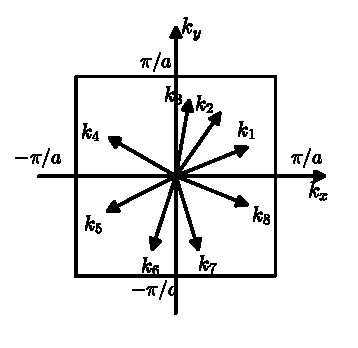
\includegraphics[width=5.5cm]{fig1-5.pdf}\\{\small 图 1.5}
\end{minipage}
\end{center}

例如二维正方点阵.BZ为正方形如图1.5，保持BZ不变的点群操作共有8个，它们是 $E$、$C_4$、$C_4^2$、$C_4^3$、$m_x$、$m_y$、$m_d$、$m_d'$，其中 $E$ 为恒等操作，$C_4$ 为垂直于纸面的4次轴，$m_x$、$m_y$ 分别为垂直于 $k_x$、$k_y$ 的对称面，$m_d$、$m_d'$ 是通过正方形两对角线的对称面.这8个元素组成的点群用 4mm 标记.

对于 BZ 中矢量 $\boldsymbol{k}_1$ 施以上述点群操作后，它将变到 $\boldsymbol{k}_1$、$\boldsymbol{k}_2$、$\cdots$、$\boldsymbol{k}_8$ 等8个点上去，这8个点在同一能带中有相同的能量
\begin{equation*}
  E_n(\boldsymbol{k}_1)=E_n(\boldsymbol{k}_2)=\cdots=E_n(\boldsymbol{k}_8)
\end{equation*}

\subsection*{2. $\boldsymbol{E}_n(\boldsymbol{k})$ 的简并度}

方程式(1.3.20)的本征值 $E_n(\boldsymbol{k})\,(n=1,2,3\cdots)$ 中可能有简并能级存在，设在 $\boldsymbol{k}$ 点第 $n$ 个能量本征值的简并度为 $d_n$，则应有 $d_n$ 个布洛赫函数 $\psi_{n,\boldsymbol{k},j}(\boldsymbol{r})\,(j=1,2,\cdots,d_n)$ 对应于同一个能量 $E_n(\boldsymbol{k})$.这种情况往往发生在BZ中某些高对称性的点与线上，这时点群中的某些元素对 $\boldsymbol{k}$ 运算后保持 $\boldsymbol{k}$ 不变（或等于 $\boldsymbol{k}+\boldsymbol{K}_n$）.这些群元对布洛赫函数作用将产生具有不同对称性的一组函数，它们同属方程式(1.3.20)的解，并且具有相同的 $\boldsymbol{k}$ 与能量 $E_n(\boldsymbol{k})$，这就是 $\psi_{n,\boldsymbol{k},j}(\boldsymbol{r})$ 的来源.为了确定能带 $E_n(\boldsymbol{k})$ 的简并度 $d_n$，人们引进 $\boldsymbol{k}$ 波矢群.

简单地说，$\boldsymbol{k}$ 波矢群就是点群 $\{\alpha|0\}$ 中使 $\boldsymbol{k}$ 不变（或变到相差倒格矢的等效点上去）的那些对称操作元素的集合所构成的群.这些操作满足条件
\begin{equation}
  \alpha\boldsymbol{k}=\boldsymbol{k}+\boldsymbol{K}_n
\end{equation}
它们组成一个点群，是 $\{\alpha|0\}$ 的子群.波矢群不可约表示的维数给出正交基函数的个数.由于同一不可约表示中各基函数有相同能量，因此 $\boldsymbol{k}$ 波矢群不可约表示的维数就等于 $\boldsymbol{k}$ 点能级的简并度 $d_n$.下面仍以二维正方点阵为例，说明如何从波矢群确定能级简并度.

又如二维正方点阵的波矢群，其BZ为正方形，保持BZ不变的对称操作属于点群 4mm，有 $E$、$C_4$、$C_4^2$、$C_4^3$、$m_x$、$m_y$、$m_d$、$m_d'$ 等8个对称操作元素.在 BZ 中有 6 个高对称性的点和线，它们是：(1)$\Gamma$、M、X 分别代表位于 BZ 中心（$\boldsymbol{k}=0$）、顶角及边界面中心的点；(2)$\Delta$、$\Sigma$、Z 分别代表位于线 $\Gamma$X、$\Gamma$M、XM 上任一点（但不包括 $\Gamma$、M、X），这6个点和线已标明于图1.6中.现在分别讨论各点的 $\boldsymbol{k}$ 波矢群及其不可约表示的维数：

\begin{center}
\begin{minipage}{5.5cm}
\centering
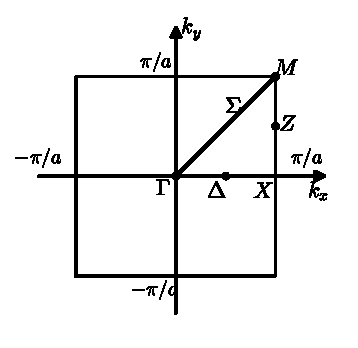
\includegraphics[width=5.5cm]{fig1-6.pdf}\\{\small 图 1.6\quad BZ 中高对称性的点与线}
\end{minipage}
\end{center}

\subsection*{(i) $\Gamma$ 点（$\boldsymbol{k}=0$）}

4mm 的 8 个对称操作均保持 $\boldsymbol{k}=0$ 不变，$\boldsymbol{k}=0$ 波矢群即点群 4mm，通常称为 $\Gamma$ 波矢群.这个群可分为5个共轭元素类，它们是：
\begin{equation*}
  E\text{、}\ C_4^2\text{、}\ C_4\text{、}C_4^3\text{、}\ m_x\text{、}m_y\text{、}\ m_d\text{、}m_d'
\end{equation*}
因此共有5个不同的不可约表示，这些表示的维数 $n_\alpha$ 应满足
\begin{equation*}
  \sum_{\alpha=1}^{5}n_\alpha^2=8
\end{equation*}
其解只可能是 $1^2+1^2+1^2+1^2+2^2=8$，说明在 $\Gamma$ 波矢群中有4个一维的和1个二维的不可约表示.因此在 $\Gamma$ 点 $E_n(0)$ 应有4种单重态和1种双重简并态.换句话说，在 $\Gamma$ 点可能有能带的二重简并发生.

\subsection*{(ii) M 点}

M 点波矢经 4mm 所有群元作用后仍在四顶角上（见图1.7），由于它们相差为倒格矢，满足条件(1.4.13)，因此 M 波矢群也是 4mm 点群，群阶 $g=8$.与 $\Gamma$ 波矢群相似，在 M 点也可能有双重简并能带出现.

\subsection*{(iii) X 点}

由于 X 点位于 $m_y$ 上，故 $m_y$ 操作不改变X，而 $m_x$ 和 $C_4^2$ 操作也只将 X 点变换到相差一倒格矢的对边中心（见图1.8）.按照式(1.4.13)，X波矢群应由 $E$、$m_x$、$m_y$、$C_4^2$ 等4个元素组成.这个群中各元素自成一个共轭类，因此有4个一维的不可约表示，说明在X点能带为非简并的.

\begin{center}
\begin{minipage}{4.5cm}
\centering
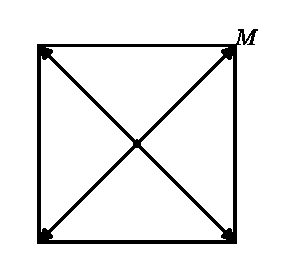
\includegraphics[width=4.5cm]{fig1-7.pdf}\\{\small 图 1.7}
\end{minipage}
\end{center}

\begin{center}
\begin{minipage}{4.5cm}
\centering
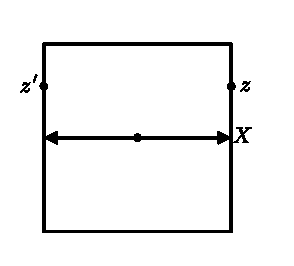
\includegraphics[width=4.5cm]{fig1-8.pdf}\\{\small 图 1.8}
\end{minipage}
\end{center}

\subsection*{(iv) $\Delta$、$\Sigma$、Z 点}

都只有两个元素组成波矢群，分别为 $\Delta$ 波矢群 $E$，$m_y$（$\Delta$ 位于 $m_y$ 上）；

$\Sigma$ 波矢群 $E$，$m_d$（$\Sigma$ 位于 $m_d$ 上）；

Z 波矢群 $E$，$m_x$[$m_x$ 操作将 $\boldsymbol{Z}\to\boldsymbol{Z}'$，两者差 $\frac{2\pi}{a}$，满足式(1.4.13)].

这些群中每个元素均自成一类，不可约表示都是一维的.在 $\Delta$、$\Sigma$、Z 上只有非简并的能带.

\subsection*{(v) BZ 中一般点 $\boldsymbol{k}_1$}

4mm 点群中除恒等元素 $E$ 外，其它7个操作将使 $\boldsymbol{k}_1$ 变为不同的波矢 $\boldsymbol{k}_2,\cdots,\boldsymbol{k}_8$（见图1.5）.波矢群只含单位元素 $E$，能带是非简并的.综上所述，在二维正方格子的布里渊区中，能带的简并只发生在BZ中心 $\Gamma$ 点与顶角M点上.

三维情况，当晶体空间群不包含滑移反映面及螺旋轴时，波矢群的分析可借助于32个点群的品格表，因为每波矢群属于32个点群之一，只需查出所对应点群品格表中恒等元素 $E$ 的特征标，即可得知波矢群不可约表示的维数，从而求得能带 $E_n(\boldsymbol{k})$ 的简并度.

到此为止，都认为对称关系
\begin{equation}
  E_n(\boldsymbol{k})=E_n(-\boldsymbol{k})
\end{equation}
是从空间反演对称性导出的.事实上，即使晶体不具空间反演对称（或换句话说，子群中不包含反演操作），例如在无对称中心的ZnS晶体中，其声子频率仍然满足式(1.4.14)，这是因为系统具有时间反演对称性.

\subsection*{3. 时间反演对称性}

时间反演是改变时间符号（$\boldsymbol{t}\to-\boldsymbol{t}$）的对称操作.由于无磁场时薛定谔方程对于时间反演操作具有不变性.因此，原来的状态和相应的时间反演态满足相同的方程，并具有同样的能量本征值.根据量子力学\textsuperscript{[3]}时间反演操作相当于：$\boldsymbol{r}\to\boldsymbol{r}$，$\boldsymbol{k}\to(-\boldsymbol{k})$ 和自旋反向 $\hat{\boldsymbol{s}}\to(-\hat{\boldsymbol{s}})$.对于晶体周期场中的单电子，当不计自旋影响时，能带用 $E_n(\boldsymbol{k})$ 表示.这样时间反演对称性即要求式(1.4.14)成立，而无需哈密顿量 $H(\boldsymbol{r})=H(-\boldsymbol{r})$——空间反演对称.将式(1.4.14)中 $E$ 换成 $\omega$，就表示声子频率的时间反演对称性.这是因为点阵力学建立在牛顿经典力学的基础上，经典力学的运动方程也具有时间反演不变性.

当考虑自旋对能谱影响时，布洛赫函数 $\psi_{n\uparrow}(\boldsymbol{k},\boldsymbol{r})$ 的时间反演态为 $\psi_{n\downarrow}(-\boldsymbol{k},\boldsymbol{r})$.量子力学已经证明，当不存在外磁场时，时间反演对称性要求上述两态满足同一个 $H$ 本征方程，并具有相同的能量本征值，这时式(1.4.14)应推广为
\begin{equation}
  E_{n\uparrow}(\boldsymbol{k})=E_{n\downarrow}(-\boldsymbol{k})
\end{equation}
这就是著名的克喇末（Kramers）定理.

值得注意的是，当晶体同时具有空间反演对称时，$E_{n\uparrow}(\boldsymbol{k})=E_{n\uparrow}(-\boldsymbol{k})$、$E_{n\downarrow}(\boldsymbol{k})=E_{n\downarrow}(-\boldsymbol{k})$ 与式(1.4.15)相结合得到
\begin{equation}
  E_{n\uparrow}(\boldsymbol{k})=E_{n\downarrow}(\boldsymbol{k})
\end{equation}
同一波矢 $\boldsymbol{k}$ 的两个不同自旋状态具有相同的能量，这一附加的两重自旋简并在固体理论中称为克喇末简并度.总之，时间反演对称性要求 $E_{n\uparrow}(\boldsymbol{k})=E_{n\downarrow}(-\boldsymbol{k})$，它是与系统的空间对称性无关的.

\section{点阵傅里叶级数}

在本节中，我们将介绍与周期性结构有关的基本数学公式，首先导出完整晶体中常用的傅里叶级数\textsuperscript{[4]}公式——点阵傅里叶级数.然后，介绍周期函数的格林定理\textsuperscript{[5]}.

\subsection*{1. 点阵傅里叶级数}

(i) 设函数 $f(\boldsymbol{r})$ 满足周期性边界条件
\begin{equation*}
  f(\boldsymbol{r})=f(\boldsymbol{r}+N_j\boldsymbol{a}_j)
\end{equation*}
其中 $\boldsymbol{a}_j\,(j=1,2,3)$ 代表正点阵基矢，$N_1N_2N_3=N$ 为元胞数，根据傅里叶展开的标准公式得到
\begin{equation}
  f(\boldsymbol{r})=(N\Omega)^{-\frac{1}{2}}\sum_{\boldsymbol{k}}f_{\boldsymbol{k}}
  \mathrm{e}^{\pm\mathrm{i}\boldsymbol{k}\cdot\boldsymbol{r}}
\end{equation}
\begin{equation}
  f_{\boldsymbol{k}}=(N\Omega)^{-\frac{1}{2}}\int_{N\Omega}\mathrm{d}\boldsymbol{r}\,
  f(\boldsymbol{r})\,\mathrm{e}^{\mp\mathrm{i}\boldsymbol{k}\cdot\boldsymbol{r}}
\end{equation}
推导式(1.5.2)时利用了关系式
\begin{equation}
  \int_{N\Omega}\mathrm{d}\boldsymbol{r}\,\mathrm{e}^{\pm\mathrm{i}\boldsymbol{k}\cdot\boldsymbol{r}}
  =(N\Omega)\,\delta_{\boldsymbol{k},0}
\end{equation}
其中 $\Omega$ 代表元胞体积，$\boldsymbol{k}$ 为满足周期性边界条件的波矢，式(1.5.1)中 $\sum_{\boldsymbol{k}}$ 是对所有的许可 $\boldsymbol{k}$ 值求和.

(ii) 设 $f(\boldsymbol{r})$ 是正点阵的周期函数
\begin{equation}
  f(\boldsymbol{r})=f(\boldsymbol{r}+\boldsymbol{l})
\end{equation}
则不难证明 $f(\boldsymbol{r})$ 可按倒格矢 $\boldsymbol{K}$ 展开为
\begin{equation}
  f(\boldsymbol{r})=\Omega^{-\frac{1}{2}}\sum_{\boldsymbol{K}}f_{\boldsymbol{K}}
  \mathrm{e}^{\pm\mathrm{i}\boldsymbol{K}\cdot\boldsymbol{r}}
\end{equation}
\begin{equation}
  f_{\boldsymbol{K}}=\Omega^{-\frac{1}{2}}\int_{\Omega}f(\boldsymbol{r})
  \mathrm{e}^{\mp\mathrm{i}\boldsymbol{K}\cdot\boldsymbol{r}}\,\mathrm{d}\boldsymbol{r}
\end{equation}
在证明上式时利用了正点阵周期函数 $f$ 的下列积分关系
\begin{equation}
\begin{aligned}
  I&=\int_{N\Omega}f(\boldsymbol{r})\mathrm{e}^{\pm\mathrm{i}\boldsymbol{k}\cdot\boldsymbol{r}}\,\mathrm{d}\boldsymbol{r}\\
  &=\sum_l\int_{\Omega}f(\boldsymbol{\rho})
  \mathrm{e}^{\pm\mathrm{i}\boldsymbol{k}\cdot(\boldsymbol{l}+\boldsymbol{\rho})}\,\mathrm{d}\boldsymbol{\rho}\\
  &=\Bigl[\sum_l\mathrm{e}^{\pm\mathrm{i}\boldsymbol{k}\cdot\boldsymbol{l}}\Bigr]
  \int_{\Omega}f(\boldsymbol{\rho})
  \mathrm{e}^{\pm\mathrm{i}\boldsymbol{k}\cdot\boldsymbol{\rho}}\,\mathrm{d}\boldsymbol{\rho}\\
  &=
  \begin{cases}
    N\displaystyle\int_{\Omega}f(\boldsymbol{\rho})
    \mathrm{e}^{\pm\mathrm{i}\boldsymbol{k}\cdot\boldsymbol{\rho}}\,\mathrm{d}\boldsymbol{\rho}
    &(\text{当 }\boldsymbol{k}=\boldsymbol{K}\text{ 倒格矢时})\\[1em]
    0&(\text{当 }\boldsymbol{k}\neq\boldsymbol{K}\text{ 时})
  \end{cases}
\end{aligned}
\end{equation}
因此，式(1.5.1)中傅里叶展开系数只取 $f_{\boldsymbol{K}}$，这就是式(1.5.5).

(iii) 当 $f$ 只在正格点 $\boldsymbol{l}$ 上定义时，式(1.5.1)直接简化为
\begin{equation}
  f(\boldsymbol{l})=(N\Omega)^{-\frac{1}{2}}\sum_{\boldsymbol{k}\in\mathrm{BZ}}f_{\boldsymbol{k}}
  \mathrm{e}^{\pm\mathrm{i}\boldsymbol{k}\cdot\boldsymbol{l}}
\end{equation}
式(1.5.8)用于晶格振动，推导时利用了 $\boldsymbol{K}\cdot\boldsymbol{l}=2\pi$（整数）.式(1.5.8)的逆傅里叶变换容易求出，将上式乘以 $N^{-\frac{1}{2}}\mathrm{e}^{\mp\mathrm{i}\boldsymbol{k}\cdot\boldsymbol{l}}$，再对 $\boldsymbol{l}$ 求和：
\begin{equation*}
\begin{aligned}
  &N^{-\frac{1}{2}}\sum_l f(\boldsymbol{l})\mathrm{e}^{\mp\mathrm{i}\boldsymbol{k}\cdot\boldsymbol{l}}\\
  &\quad=\Omega^{-\frac{1}{2}}\sum_{\boldsymbol{k}'\in\mathrm{BZ}}f_{\boldsymbol{k}'}
  \Bigl\{\frac{1}{N}\sum_l\mathrm{e}^{\pm\mathrm{i}(\boldsymbol{k}'-\boldsymbol{k})\cdot\boldsymbol{l}}\Bigr\}\\
  &\quad=\Omega^{-\frac{1}{2}}\sum_{\boldsymbol{k}'\in\mathrm{BZ}}f_{\boldsymbol{k}'}
  \delta_{\boldsymbol{k},\boldsymbol{k}'}=\Omega^{-\frac{1}{2}}f_{\boldsymbol{k}}
\end{aligned}
\end{equation*}
因此
\begin{equation}
  f_{\boldsymbol{k}}=\left(\frac{\Omega}{N}\right)^{\frac{1}{2}}\sum_l f(\boldsymbol{l})
  \mathrm{e}^{\mp\mathrm{i}\boldsymbol{k}\cdot\boldsymbol{l}}
\end{equation}
(iv) 当 $f$ 是 $\boldsymbol{k}$ 空间的函数，并满足
\begin{equation}
  f(\boldsymbol{k})=f(\boldsymbol{k}+\boldsymbol{K})
  \qquad(\boldsymbol{K}\ \text{是倒格矢})
\end{equation}
时，若令式(1.5.8)和(1.5.9)中
\begin{equation*}
  \Omega^{-\frac{1}{2}}f_{\boldsymbol{k}}\to f(\boldsymbol{k})
\end{equation*}
则得到关系式
\begin{equation}
  f(\boldsymbol{k})=N^{-\frac{1}{2}}\sum_l f(\boldsymbol{l})
  \mathrm{e}^{\mp\mathrm{i}\boldsymbol{k}\cdot\boldsymbol{l}}
\end{equation}
和
\begin{equation}
  f(\boldsymbol{l})=N^{-\frac{1}{2}}\sum_{\boldsymbol{k}\in\mathrm{BZ}}f(\boldsymbol{k})
  \mathrm{e}^{\pm\mathrm{i}\boldsymbol{k}\cdot\boldsymbol{l}}
\end{equation}
式(1.5.11)就倒点阵周期函数按正格矢 $\boldsymbol{l}$ 展开的点阵傅里叶级数，用于瓦尼尔（Wannier）函数.

\subsection*{2. 周期函数的格林定理}

设 $u(\boldsymbol{r})$ 与 $v(\boldsymbol{r})$ 均为正点阵的周期函数，则下列等式成立
\begin{equation}
  \int_{\Omega}\mathrm{d}\tau\,u\,\nabla v
  =-\int_{\Omega}\mathrm{d}\tau\,v\,\nabla u
\end{equation}
\begin{equation}
  \int_{\Omega}\mathrm{d}\tau\,u\nabla^2v
  =\int_{\Omega}\mathrm{d}\tau\,v\nabla^2u
\end{equation}
其中 $\Omega$ 为元胞体积，式(1.5.13)和(1.5.14)可称为周期函数的格林定理.

[证明]设 $f(\boldsymbol{r})$ 为任意函数，具有正点阵的周期性，它在元胞 $\Omega$ 内的积分
\begin{equation}
  I(\boldsymbol{r}')=\int_{\Omega}\mathrm{d}\tau\,f(\boldsymbol{r}+\boldsymbol{r}')
\end{equation}
应与 $\boldsymbol{r}'$ 无关，因此 $I(\boldsymbol{r}')$ 对 $\boldsymbol{r}'$ 的一、二阶导数必为零，于是有关系式
\begin{equation}
  \nabla'I(\boldsymbol{r}')
  =\int_{\Omega}\mathrm{d}\tau\,\nabla'f(\boldsymbol{r}+\boldsymbol{r}')
  =\int_{\Omega}\mathrm{d}\tau\,\nabla f(\boldsymbol{r}+\boldsymbol{r}')=0
\end{equation}
\begin{equation}
  \nabla'^2I(\boldsymbol{r}')
  =\int_{\Omega}\mathrm{d}\tau\,\nabla'^2f(\boldsymbol{r}+\boldsymbol{r}')
  =\int_{\Omega}\mathrm{d}\tau\,\nabla^2 f(\boldsymbol{r}+\boldsymbol{r}')=0
\end{equation}
再令 $\boldsymbol{r}'=0$，则求得周期函数 $f(\boldsymbol{r})$ 满足
\begin{equation}
  \int_{\Omega}\mathrm{d}\tau\,\nabla f(\boldsymbol{r})=0
\end{equation}
\begin{equation}
  \int_{\Omega}\mathrm{d}\tau\,\nabla^2 f(\boldsymbol{r})=0
\end{equation}
若假设
\begin{equation}
  f(\boldsymbol{r})=u(\boldsymbol{r})v(\boldsymbol{r})
\end{equation}
代入式(1.5.18)，即求得式(1.5.13)，代入式(1.5.19)有
\begin{equation}
  \int_{\Omega}\mathrm{d}\tau\bigl[u\nabla^2v+v\nabla^2u
  +2\nabla u\cdot\nabla v\bigr]=0
\end{equation}
再设 $v$ 与 $\nabla u$ 组成式(1.5.13)中两个周期函数，可得关系式
\begin{equation}
  2\int_{\Omega}\mathrm{d}\tau\,\nabla u\cdot\nabla v
  =-2\int_{\Omega}\mathrm{d}\tau\,u\,\nabla^2v
\end{equation}
将式(1.5.22)代入式(1.5.21)即证明了式(1.5.14).

周期函数的格林定理在能带理论中有重要应用.

\begin{canKao}
\begin{enumerate}[label={[\arabic*]}, leftmargin=2.2em, itemsep=0pt]
\item Morgan D J. Group Theory and Electron State in Perfect Crystals. In: Landsberg P T, ed. Solid State Theory. London: Wiley-Interscience, 1969
\item Callaway J. Quantum Theory of Solid State. New York: Academic Press, 1976. Chap 3
\item Merzbacher E. Quantum Mechanics (2nd ed). New York: John Wiley and Sons Inc, 1970. Chap 16
\item Landsberg P T. Solid State Theory. London: Wiley-Interscience, 1969. Chap 2
\item Aschroft N W, Mermin N D. Solid State Physics. New York: Holt, Rinehart and Winston, 1976
\end{enumerate}
\end{canKao}
